% Chapter 1

\chapter{Introduction} % Main chapter title
\label{Chapter1} % For referencing the chapter elsewhere, use \ref{Chapter1} 

\lhead{Chapter 1. \emph{Introduction}} % This is for the header on each page - perhaps a shortened title

%----------------------------------------------------------------------------------------
% Section 1
%----------------------------------------------------------------------------------------

\section{Context}

\Gls{ml} algorithms are becoming increasingly present in systems that operate within shared environments
with humans, or involve direct interaction with humans themselves~\citep{pereira}. These systems 
are often defined as safety-critical, such that their failures lead to unintended and potentially harmful behaviours~\citep{amodei}.
Examples of these systems include autonomous automotive systems, traffic control systems, medical devices, aviation software, industrial robotics, and many more cyber-physical systems that interact with our environment.
Many of these systems have so far only existed as proof of concepts, but are steadily approaching commercial use within our society.
Consequently, the safety of \gls{ml} for the use of controlling safety critical systems has become a focused area of research in recent years.

The issue regarding \gls{ml} within safety-critical systems stems from the typically stochastic nature of their algorithms, which
leads to a lower degree of understanding than software that is explicitly programmed to perform a specific task~\citep{bishop}.

Additionally, recent research has exposed broad vulnerabilities within data driven \gls{ml} algorithms, including \Glspl{nn}; where applying 
small but intentional perturbations to an input which are not noticble to humans,
can lead to a model outputting an incorrect classification with high confidence.~\citep{goodfellow}.
An example of such an attack can be seen in \textit{Fig.~\ref{fig:adversarialpatch}} below.

\begin{figure}[H]
	\centering
        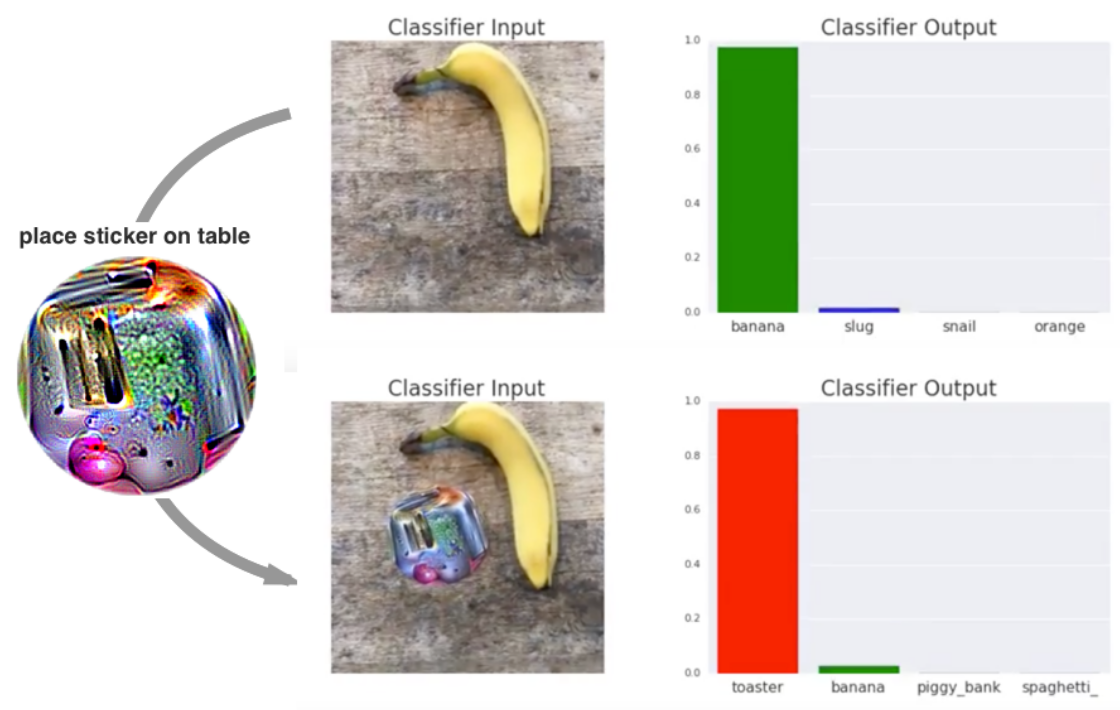
\includegraphics[width=1.0\textwidth]{media/introduction/sticker.png}
        \rule{35em}{0.5pt}
        \caption[Google's Aversarial Patch]{\textbf{Google's Adversarial Patch} -- An example of a method to create targeted adversarial attacks on \glspl{nn} by adding carefully designed noise via a physical patch~\citep{brown2018}.}\label{fig:adversarialpatch}
\end{figure}

Various languages have been developed over time that have either been exetended to, or have been intentionally designed to handle formal
approaches to verifying software (Ada, Haskell etc.). However, few of these languages have been adopted by the \gls{ml} community, and therefore
there is a trade off decision that needs to be made; choose a language that is efficient and easy for developers to create \gls{ml} models,
or a language that allows developers to produce robust and verified models.
% Section about different programming languages for ml



\section{Motivation}


Software engineers are often limited to what programming languages they can choose from to develop a project. This could be
due to the constraints of a wider system used by their employer, or that their preferred language is not suitable for 
a specific task. This is especially true for developing \gls{ml} that can be formally verified, partly because of the relatively
new area of research, but also because languages adopted for \gls{ml} are not as well equipped for formal verification methods. Therefore, there is a need
for a generalised approach for verifying \gls{ml} models accross a wider range of programming languages.

Talk about the recent machine learning advancements in Go, and that it has shown to be used for machine learning in infrastructure, and could be 
adopted as a language for verification of neural networks.

\section{Aims \& Objectives}
